\documentclass[11pt]{amsart}
\usepackage[margin=1.15in]{geometry}
\usepackage{amssymb,mathtools,booktabs,graphicx,microtype,flafter}
\usepackage[hidelinks]{hyperref}

\newtheorem{theorem}{Theorem}[section]
\newtheorem{proposition}[theorem]{Proposition}
\newtheorem{lemma}[theorem]{Lemma}
\newtheorem{corollary}[theorem]{Corollary}
\theoremstyle{definition}
\newtheorem{definition}[theorem]{Definition}
\newtheorem{conjecture}[theorem]{Conjecture}
\newtheorem{observation}[theorem]{Numerical result}
\theoremstyle{remark}
\newtheorem{remark}[theorem]{Remark}

\newcommand{\C}{\mathbb{C}}
\newcommand{\D}{\mathbb{D}}
\newcommand{\Z}{\mathbb{Z}}
\newcommand{\Q}{\mathbb{Q}}
\newcommand{\PP}{\mathcal{P}_0}
\newcommand{\NF}{\mathcal{N}}
\newcommand{\Mf}{\mathcal{M}}
\newcommand{\cG}{\mathcal{G}}
\newcommand{\fa}[1]{f_{e^{2\pi i#1}}}
\newcommand{\Res}{\operatorname*{Res}}
\newcommand{\resit}{\operatorname{r\acute{e}sit}}

\begin{document}

\title[Beyond the Ford-circle law (abridged)]{Beyond the Ford-circle law:\\ parabolic renormalization and the shape\\ of Mandelbrot satellite bulbs\\[0.4ex] {\normalsize\mdseries (abridged version)}}
\author{Lars Bendixen}
\date{September 2026}
\subjclass[2020]{Primary 37F46; Secondary 37F25, 37F10}
\keywords{Mandelbrot set, satellite components, Ford circles, holomorphic index, horn map, parabolic renormalization}

\begin{abstract}
The main cardioid of the Mandelbrot set carries a ``bulb'' (a satellite component) at every rational internal angle $p/q$. To leading order the bulb at $p/q$ is a round disc of diameter $2\sin(\pi p/q)/q^2$, which is the scaling of the Ford circles of number theory. We study how the bulbs deviate from this picture. A bulb is described by the multiplier of its attracting cycle. In the rescaled parameter $u=q^2\varepsilon$ this multiplier begins $1-u$ for every bulb, which is the Ford law. The first coefficient that distinguishes bulbs, $\kappa(p/q)$, measures how far the bulb is from round. We prove that $\kappa(p/q)=(\iota_{p/q}-\frac12)/q$, where $\iota_{p/q}$ is the holomorphic index of the parabolic fixed point from which the bulb is born, and we give an efficient recursion for it. The rest of the work is numerical. It shows that $\kappa$ is controlled by parabolic renormalization, which zooms in on the parabolic point and returns a new map, its horn map. For the bulbs at angles $1/q$, $\kappa$ tends to a new constant $\kappa_0\approx0.02383-0.05230\,i$. This is the index of the horn map of $z+z^2$, and the two agree to $24$ digits. The same mechanism, combined with an exactly computable phase, predicts the bulb sizes and the whole first-order correction in $1/q$. Repeating the renormalization along continued fractions gives constants that converge to a limit $\kappa_*$. At each rational tested, the bulbs approaching it from above and from below have different limits, given by the two horn maps of the parabolic point there; we conjecture that this holds at every rational. The bulbs of other components, and those of the family $z^3+c$, follow the same principle with their own parabolic germs.
\end{abstract}

\maketitle

\section{Introduction}
Let $c(\lambda)=\lambda/2-\lambda^2/4$ parametrize the main cardioid of the Mandelbrot set by the multiplier $\lambda\in\D$ of its attracting fixed point; equivalently we use $f_\lambda(z)=\lambda z+z^2$. At $\lambda_0=e^{2\pi ip/q}$ the satellite $W_{p/q}$ of period $q$ is attached~\cite{DH}. Its size is of order $q^{-2}$~\cite{GM}, and to first order it is a disc of diameter $2|c'(\lambda_0)|q^{-2}=2\sin(\pi p/q)\,q^{-2}$~\cite{FM}. Up to the factor $\sin(\pi p/q)$ these are the Ford circles~\cite{Ford}. We study the first correction to this law.

Put $\lambda=\lambda_0e^\varepsilon$, let $\rho_{p/q}(\varepsilon)$ be the multiplier of the $q$-cycle that bifurcates from $0$, and write
\begin{equation}\label{eq:R}
R_{p/q}(u):=\rho_{p/q}(u/q^2)=\sum_{k\ge0}r_k(p/q)\,u^k .
\end{equation}
Up to a conformal change of variable, $W_{p/q}=\{|R_{p/q}|<1\}$. We show that $r_0=1$ and $r_1=-1$ for all $p/q$, so that to first order $W_{p/q}$ is the disc $|u-1|<1$; this is the Ford law. The first coefficient that depends on $p/q$ is $\kappa(p/q):=r_2(p/q)$, and it governs the leading deviation of $W_{p/q}$ from a disc. The bulb size is measured by $G(p/q)=\frac12|u_a|\,(1+O(q^{-2}))$, where $R_{p/q}(u_a)=-1$ and $G=1$ to first order.

\emph{Results.} Section~\ref{sec:exact} contains the proved statements: the index formula for $\kappa$, and a normal form that computes it in $O(q^2)$ operations. The remaining sections are numerical, and each claim is stated as a conjecture together with its evidence. We find that, up to $O(q^{-2})$, the bulb is described by the near-parabolic renormalization of $f_{\lambda_0}$ in the sense of Inou and Shishikura~\cite{IS}, composed with an exact phase. This picture yields five constants, collected in Table~\ref{tab:constants}. The full version~\cite{full} contains proofs omitted here, degree-three details, error analysis and data; all code and data are in~\cite{repo}.

\begin{table}[t]
\centering\footnotesize
\begin{tabular}{@{}lllll@{}}
\toprule
constant & germ & value & bulbs & \\
\midrule
$\kappa_0$ & $z+z^2$ & $0.02382588740220057 - 0.05230465911400367\,i$ & $3\cdot10^{-28}$ & \S\ref{sec:horn} \\
$\kappa_0^{(3)}$ & $v+v^2+\frac13v^3$ & $0.1435992780952916 - 0.03031164789850254\,i$ & $1.3\cdot10^{-6}$ ($q=1024$) & \S\ref{sec:degree3} \\
$\kappa_{1/2}$ & $-z+z^2$ & $0.01840526161796478 - 0.04290372388023048\,i$ & $3\cdot10^{-10}$ & \S\ref{sec:component} \\
$\kappa_*$ & $G_*=\mathcal P(\bar G_*)$ & $0.011929183413 - 0.037455493752\,i$ & levels $\le3$ & \S\ref{sec:hierarchy} \\
$G_0$ & $e^{u}\mathcal P_0$ & $1.02641539$ & $4\cdot10^{-8}$ & \S\ref{sec:unfolding} \\
\bottomrule
\end{tabular}

\caption{The constants. ``Bulbs'' is the difference between the horn-map value and the best extrapolated bulb limit ($\kappa_0^{(3)}$: error at $q=1024$, decaying like $q^{-2}$). The extrapolation uncertainties are about $3\cdot10^{-25}$ for $\kappa_0$, $2\cdot10^{-7}$ for $\kappa^+_{1/2}$ and $10^{-6}$ for $G_0$.}\label{tab:constants}
\end{table}

\section{Exact results}\label{sec:exact}
Write $f=f_{\lambda_0}$. The fixed point $0$ has a single cycle of $q$ petals, so $f^q(z)=z+az^{q+1}+O(z^{q+2})$ with $a\ne0$. Let $\iota_{p/q}=\Res_{z=0}dz/(z-f^q(z))$ be its holomorphic index~\cite{Milnor}.

\begin{theorem}[Index formula]\label{thm:index}
$\rho_{p/q}(\varepsilon)=1-q^2\varepsilon+q^3(\iota_{p/q}-\frac12)\varepsilon^2+O(\varepsilon^3)$. Equivalently, $r_0=1$, $r_1=-1$ and $\kappa(p/q)=(\iota_{p/q}-\frac12)/q$.
\end{theorem}

\begin{proof}[Sketch]
For small $\varepsilon\ne0$, $f^q_\lambda$ has $q+1$ simple fixed points near $0$: the point $0$, with multiplier $e^{q\varepsilon}$, and one $q$-cycle, with multiplier $\rho$. The sum of their indices converges to $\iota_{p/q}$, which gives
\[
\frac1{1-e^{q\varepsilon}}+\frac q{1-\rho(\varepsilon)}\longrightarrow\iota_{p/q}.
\]
The first term is $-1/(q\varepsilon)+\frac12+O(\varepsilon)$. Boundedness of the sum forces $1-\rho=q^2\varepsilon+O(\varepsilon^2)$, and the constant term gives the coefficient of $\varepsilon^2$.
\end{proof}

The proof uses only the multiplicity $q+1$, so it applies to the satellites of every hyperbolic component of $z^d+c$, with the first-return map in place of $f$. Since $f^q$ has coefficients in $\Z[\lambda_0]$, $\kappa(p/q)\in\Q(\zeta_q)$, and the values $\kappa(p'/q)$ form a Galois orbit; for instance $\kappa(\frac12)=-\frac3{16}$ and $\kappa(\frac13)=(-241-16\sqrt3\,i)/2646$.

\begin{theorem}[Normal form]\label{thm:nf}
Let $\NF(z)=\lambda_0z(1+b_1z^q+b_2z^{2q})$ be the resonant normal form of $f$ to order $2q+1$. Its coefficients satisfy an explicit triangular recursion of cost $O(q^2)$, and
\[
a=qb_1,\qquad\kappa(p/q)=\frac12-\frac1{2q}-\frac1{2q^2}+\frac{b_2}{(qb_1)^2}=\iota(Q_{p/q})-\frac12,
\]
where $Q_{p/q}(W)=\NF^q(W^{1/q})^q$ is the rotation quotient of $\NF^q$.
\end{theorem}

Composing $f$ symbolically $q$ times costs $O(q^3)$ and suffers severe cancellation, since $|a(1/q)|$ grows like $(q/2\pi)^q$. The recursion is stable; in Arb ball arithmetic~\cite{Arb} it certifies $\kappa(1/q)$ for $q\le32768$.

\section{The horn map of $z+z^2$ and $\kappa_0$}\label{sec:horn}
Let $E(Z)=\Phi_{\rm att}\circ\Psi_{\rm rep}(Z)=Z+\sum_{n\ge1}a_ne^{2\pi inZ}$ be the upper horn map of $f_1(z)=z+z^2$, with the standard normalization $a_0=0$~\cite{Lavaurs,Sh}. Let
\[
\PP(W)=W\exp\Bigl(2\pi i\sum_{n\ge1}a_nW^n\Bigr)
\]
be its parabolic renormalization~\cite{IS,LY}.

\begin{lemma}\label{lem:hornindex}
$\iota(\PP)-\frac12=a_2/(2\pi ia_1^2)$, independently of the normalization of the Fatou coordinates.
\end{lemma}

\begin{proof}
$\PP(W)=W+AW^2+BW^3+\dots$ with $A=2\pi ia_1$ and $B=2\pi ia_2+\frac12A^2$, and $\iota=B/A^2$. A translation of both Fatou coordinates by $\tau$ sends $a_n\mapsto a_ne^{2\pi in\tau}$, which leaves $a_2/a_1^2$ unchanged.
\end{proof}

\begin{observation}\label{obs:kappa0}
The horn map, computed from exact Fatou series at $60$ and $80$ digits, gives
\begin{align*}
\operatorname{Re}\kappa_0&=\phantom{-}0.023825887402200569000729189645402,\\
\operatorname{Im}\kappa_0&=-0.052304659114003666316522486207571,
\end{align*}
where $\kappa_0:=\iota(\PP)-\frac12$.
Least-squares fits $\kappa(1/q)=\sum_{j\le10}\gamma_jq^{-j}$ over certified values $256\le q\le32768$ give $\gamma_0$ equal to this value to $3\cdot10^{-28}$, and $\gamma_1=-i/(2\pi)$ to $2\cdot10^{-23}$. Other stable fits move $\gamma_0$ by at most $3\cdot10^{-25}$.
\end{observation}

\begin{conjecture}\label{conj:main}
$\kappa(1/q)=\kappa_0-\dfrac{i}{2\pi q}+O(q^{-2})$.
\end{conjecture}

\begin{figure}[t]
\centering
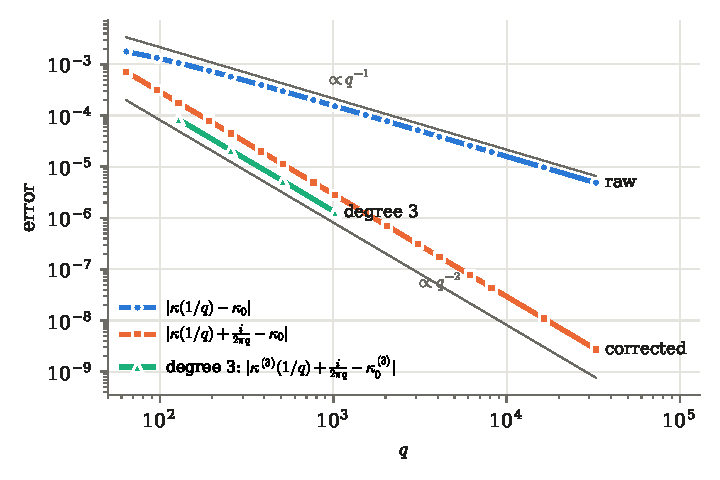
\includegraphics[width=0.72\textwidth]{figures/convergence.pdf}
\caption{$\kappa(1/q)\to\kappa_0$ (degree two) and $\kappa^{(3)}(1/q)\to\kappa_0^{(3)}$ (degree three). After the universal correction $-i/(2\pi q)$ the error decays like $q^{-2}$.}\label{fig:conv}
\end{figure}

\section{The renormalization principle}\label{sec:renorm}
Near-parabolic renormalization $\mathcal R$~\cite{IS} assigns to $\fa{\alpha}$ a germ with multiplier $e^{-2\pi i/\alpha}$, and parabolic implosion~\cite{Lavaurs,Sh} identifies its limits with $\PP$ times a phase. The phase is exact.

\begin{proposition}[Kinematics]\label{prop:kinematic}
If $e^{2\pi i\alpha}=\lambda_0e^{u/q^2}$, then $e^{-2\pi i/\alpha}=e^{-2\pi iq/p}\,e^{\tilde u/p^2}$ with $\tilde u=u/\bigl(1+u/(2\pi ipq)\bigr)$.
\end{proposition}

\begin{proof}
$\alpha=(2\pi ipq+u)/(2\pi iq^2)$, and $2\pi ip^2(q/p-1/\alpha)=\tilde u$.
\end{proof}

Fix $p$ and $r$ coprime, let $q=pN+r$, $\mu=e^{-2\pi ir/p}$, and let $\rho_{p,r}(u)$ be the multiplier of the $p$-cycle of $\Mf_u=\mu e^{u/p^2}\PP$ that bifurcates from $0$.

\begin{conjecture}[Renormalization principle]\label{conj:unfolding}
$R_{p/q}(u)=\rho_{p,r}(\tilde u(u))+O(q^{-2})$ coefficientwise, and uniformly on a neighbourhood of the arc from $0$ to the point where $\rho_{p,r}=-1$.
\end{conjecture}

Comparing coefficients gives $\kappa(p/q)=\kappa_{p,r}-i/(2\pi pq)+O(q^{-2})$, where
\begin{equation}\label{eq:boundedp}
\kappa_{p,r}=\frac{\iota\bigl((\mu\PP)^p\bigr)-\frac12}{p},
\end{equation}
by Theorem~\ref{thm:index} applied to $\mu e^\varepsilon\PP$. The first-order term involves no property of the germ.

\emph{Evidence.} In all nine classes with $2\le p\le5$, \eqref{eq:boundedp} agrees with the extrapolated bulb limits to between $6\cdot10^{-9}$ and $2.6\cdot10^{-8}$, within the extrapolation uncertainty. The opposite phase fails.

\label{sec:unfolding}The predicted bulb sizes agree with the bulbs to $9\cdot10^{-7}$ in all ten classes with $p\le5$. For $p=1$ this gives diameters $2\pi G_0q^{-3}(1+O(q^{-1}))$ for the $1/q$-bulbs at the cusp, with $G_0=1.02641539\ldots$.

For $2\le k\le8$, $(p,r)\in\{(1,1),(2,1),(3,1),(3,2)\}$ and $N=64,\dots,1024$, the residuals $|r_k(p/q)-[u^k]\rho_{p,r}(\tilde u)|$ fall by a factor $3.8$--$4.3$ per doubling of $N$, that is, like $q^{-2}$. Without $u\mapsto\tilde u$ the factor is only $1.1$--$2.0$ (Figure~\ref{fig:kinematic}). Numerically, then, the entire $O(1/q)$ part of $R_{p/q}$ is kinematic.

\begin{figure}[t]
\centering
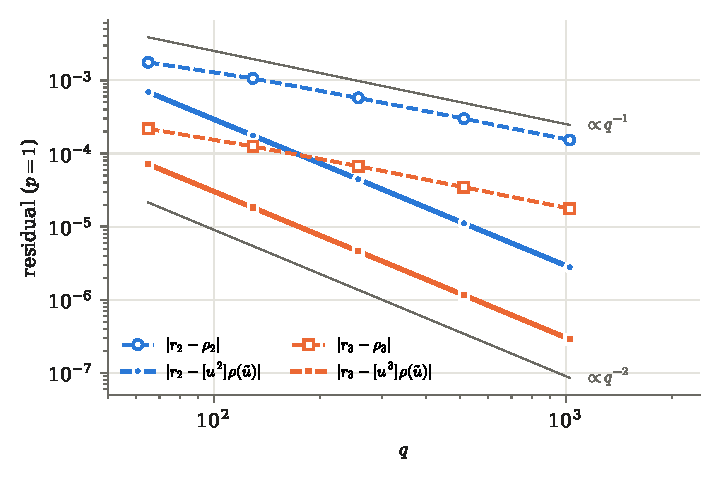
\includegraphics[width=0.72\textwidth]{figures/kinematic.pdf}
\caption{Residuals of $r_2,r_3$ of $R_{1/q}$ against the renormalized family, with (solid) and without (dashed) the M\"obius substitution $u\mapsto\tilde u$.}\label{fig:kinematic}
\end{figure}

\section{The hierarchy and $\kappa_*$}\label{sec:hierarchy}
The renormalization $\mathcal R$ acts on continued fractions as the Gauss map, after conjugation by $z\mapsto\bar z$. Therefore, when the first $k$ partial quotients are large, each renormalization should be close to $\mathcal P$ applied to the complex conjugate of the previous one. Normalize germs to $v+v^2+O(v^3)$, write $\bar\cG(W)=\overline{\cG(\bar W)}$, and put
\[
\cG_1=\mathcal P(f_1),\qquad\cG_{k+1}=\mathcal P(\bar\cG_k),\qquad\kappa_k=\iota(\cG_k)-\tfrac12 .
\]

\begin{observation}\label{obs:kstar}
Two independent settings agree to $2\cdot10^{-14}$ for $k\le7$. The differences $\kappa_{k+1}-\kappa_k$ contract antilinearly, $\Delta\mapsto\nu\bar\Delta$ with $|\nu|=0.0419$. This is the signature of the antilinear derivative of $\cG\mapsto\mathcal P(\bar\cG)$. Extrapolation gives
\[
\kappa_*=\lim_k\kappa_k=0.011929183413-0.037455493752\,i .
\]
Without the conjugation our code reproduces the fixed point of Lanford and Yampolsky~\cite{LY}: cubic coefficient $0.5142768-0.0346276\,i$, eigenvalue ratio $-0.01764+0.04038\,i$. That operator, however, does not govern the bulbs.
\end{observation}

\begin{conjecture}\label{conj:hierarchy}
$\lim_{N_k\to\infty}\cdots\lim_{N_1\to\infty}\kappa([0;N_1,\ldots,N_k])$ equals $\kappa_k$ for $k$ odd and $\overline{\kappa_k}$ for $k$ even.
\end{conjecture}

This holds numerically for $k\le3$. At $k=2$ the bounded-$p$ route gives $\overline{\kappa_2}$ to $1.2\cdot10^{-8}$, and the diagonal $[0;N,N]$ gives it to $3\cdot10^{-10}$. At $k=3$ the diagonal $[0;N,N,N]$, with $q\le64080$, gives $\kappa_3$ to $10^{-5}$, while $|\kappa_3-\kappa_2|=7.8\cdot10^{-4}$.

\section{Limits at parabolic roots}\label{sec:component}
Let $p/q=[0;a_1,\ldots,a_\ell]$, using either of its two continued-fraction expansions. Let $\tau$ be a fixed tail with $[0;\tau]=r_\tau/p_\tau$, where $r_\tau=0$ and $p_\tau=1$ for $\tau=\varnothing$. As $N\to\infty$ the satellites $[0;a_1,\ldots,a_\ell,N,\tau]$ approach the root of $W_{p/q}$, from above if $\ell$ is even and from below if $\ell$ is odd. There the cusp germ is replaced by the $q$-petal germ $\fa{p/q}(z)=e^{2\pi ip/q}z+z^2$.

The construction of Section~\ref{sec:horn} extends to $g=\fa{p/q}^q$. There is a formal Fatou coordinate
\[
\Phi=-z^{-q}/(qa)+\sum s_kz^k+\beta\log z,
\]
where $\beta=\resit(g)=\frac{q+1}2-\iota(g)$; this follows from a residue computation. The orbits from a repelling petal above or below an escape band land in different attracting petals, and are carried back by $f^m$ with $m\equiv-jp^{-1}\pmod q$. This defines an upper and a lower horn map, with germs $\mathcal P^\pm_{p/q}$ normalized tangent to the identity. Put $\kappa^\pm_{p/q}=\iota(\mathcal P^\pm_{p/q})-\frac12$. Then $\kappa^\pm_{0/1}=\kappa_0,\overline{\kappa_0}$ and $\kappa^-_{p/q}=\overline{\kappa^+_{(q-p)/q}}$, but for $q\ge3$ the constants $\kappa^+_{p/q}$ and $\kappa^-_{p/q}$ at the same $p/q$ are not conjugate.

\begin{conjecture}[Root limits]\label{conj:rational}
Let $\mu_\tau=e^{-2\pi ir_\tau/p_\tau}$. From above,
\[
\lim_{N\to\infty}\kappa([0;a_1,\ldots,a_\ell,N,\tau])=\frac{\iota\bigl((\mu_\tau\mathcal P^+_{p/q})^{p_\tau}\bigr)-\frac12}{p_\tau}.
\]
From below the same formula holds with $\overline{\mu_\tau}\,\mathcal P^-_{p/q}$ in place of $\mu_\tau\mathcal P^+_{p/q}$. In particular $\kappa$ has the distinct one-sided limits $\kappa^\pm_{p/q}$ at every rational.
\end{conjecture}

The conjugate phase from below is forced by $\kappa(1-x)=\overline{\kappa(x)}$. Table~\ref{tab:rational} tests the conjecture in fifteen cases. Eight have $\tau=\varnothing$, at $\frac13,\frac14,\frac25,\frac37$ from both sides. Seven have tails with $p_\tau=2,3$, at $\frac13$, $\frac12$ and $\frac11$; four of these approach from below with a non-real phase. All agree to $6\cdot10^{-11}$. At $\frac13$, for instance, $\kappa^-_{1/3}=0.0158408+0.0401752\,i$ and $\kappa^+_{1/3}=0.0165812-0.0395047\,i$.

\begin{table}[t]
\centering\scriptsize
\begin{tabular}{@{}lllllc@{}}
\toprule
$p/q$ & side & $\tau$ & horn map of $e^{2\pi ip/q}z+z^2$ & bulbs, extrapolated & $|\Delta|$ \\
\midrule
$1/3$ & below & $\varnothing$ & $0.015840773234 + 0.040175221242\,i$ & $0.015840773241 + 0.040175221243\,i$ & $6.5\cdot10^{-12}$ \\
$1/3$ & above & $\varnothing$ & $0.016581162594 - 0.039504714589\,i$ & $0.016581162601 - 0.039504714589\,i$ & $6.4\cdot10^{-12}$ \\
$1/4$ & below & $\varnothing$ & $0.014455842876 + 0.039068895117\,i$ & $0.014455842881 + 0.039068895118\,i$ & $5.3\cdot10^{-12}$ \\
$1/4$ & above & $\varnothing$ & $0.015760467204 - 0.037801851383\,i$ & $0.015760467209 - 0.037801851382\,i$ & $5.3\cdot10^{-12}$ \\
$2/5$ & below & $\varnothing$ & $0.014434584508 + 0.037505178012\,i$ & $0.014434584513 + 0.037505178012\,i$ & $4.6\cdot10^{-12}$ \\
$2/5$ & above & $\varnothing$ & $0.014296912442 - 0.037686119109\,i$ & $0.014296912446 - 0.037686119110\,i$ & $4.6\cdot10^{-12}$ \\
$3/7$ & above & $\varnothing$ & $0.013301284920 - 0.037190044710\,i$ & $0.013301284861 - 0.037190044712\,i$ & $5.9\cdot10^{-11}$ \\
$3/7$ & below & $\varnothing$ & $0.013998687363 + 0.036367863348\,i$ & $0.013998687363 + 0.036367863334\,i$ & $1.4\cdot10^{-11}$ \\
$1/3$ & above & $2$ & $0.046849904480 - 0.018242741860\,i$ & $0.046849904482 - 0.018242741860\,i$ & $2.7\cdot10^{-12}$ \\
$1/3$ & below & $2$ & $0.046510029333 + 0.018510459943\,i$ & $0.046510029336 + 0.018510459943\,i$ & $2.8\cdot10^{-12}$ \\
$1/3$ & above & $3$ & $0.052913142048 - 0.001728643502\,i$ & $0.052913142050 - 0.001728643502\,i$ & $1.7\cdot10^{-12}$ \\
$1/2$ & below & $3$ & $0.053307011907 + 0.002605955801\,i$ & $0.053307011909 + 0.002605955801\,i$ & $2.5\cdot10^{-12}$ \\
$1/3$ & below & $3$ & $0.052713652883 + 0.001878998752\,i$ & $0.052713652885 + 0.001878998752\,i$ & $1.7\cdot10^{-12}$ \\
$1/1$ & below & $3$ & $0.054529447219 + 0.005017189409\,i$ & $0.054529447226 + 0.005017189408\,i$ & $6.7\cdot10^{-12}$ \\
$1/3$ & below & $(1,2)$ & $0.053167372528 + 0.020247303769\,i$ & $0.053167372529 + 0.020247303768\,i$ & $1.6\cdot10^{-12}$ \\
\bottomrule
\end{tabular}

\caption{One-sided limits of $\kappa$ at rationals: the tail rule of Conjecture~\ref{conj:rational} against the bulbs $[0;a_1,\ldots,a_\ell,N,\tau]$, extrapolated from $N=128,\ldots,2048$ (degree four against degree three: at most $1.3\cdot10^{-9}$).}\label{tab:rational}
\end{table}

\emph{Other components.} For a hyperbolic component $W$, call the first-return map of the parabolic cycle at its root the \emph{root germ} of $W$. We conjecture (the root principle) that the limits of $\kappa$ and of $G$ along the satellites of $W$ at angles $[0;N,\tau]$ and $1-[0;N,\tau]$ are given by the rule above, with the upper and lower horn germs of the root germ. We tested this for the following components:
\begin{itemize}
\item the period-two disc: its root germ is $\fa{1/2}$, and its constant $\kappa^+_{1/2}$ is known to $32$ digits, and the best bulb fits agree with it to $2\cdot10^{-9}$ (uncertainty $2\cdot10^{-7}$);
\item the period-three disc $W_{1/3}$: both sides follow $\mathcal P^\pm_{1/3}$, and the other three candidate germs miss by $10^{-3}$ or more;
\item the real period-three component, whose root is a cusp with root germ normalized to $v+v^2-\frac2{49}v^3+\dots$ (exactly): agreement to $4\cdot10^{-10}$, with a kinematic first-order term;
\item a period-six component at the $\frac13$-root of the period-two disc.
\end{itemize}
At that last root the root germ is not formally conjugate to $\fa{1/3}$. Its root index differs by $6\cdot10^{-2}$, yet its horn constants differ from $\kappa^\pm_{1/3}$ by only about $1.5\cdot10^{-4}$, and the satellites follow its own constants.

\section{Degree three and outlook}\label{sec:degree3}
For $z^3+c$, near the cusp of the main component, the germ is $v+v^2+\frac13v^3$. Its horn map gives $\kappa_0^{(3)}=0.1435992780952916-0.0303116478985025\,i$, and $\kappa^{(3)}(1/q)+i/(2\pi q)\to\kappa_0^{(3)}$ like $q^{-2}$. The universal first-order term is unchanged and the constant is not. Here each bulb has two points of multiplier $-1$, and both of their sizes are predicted. Integer-relation searches (PSLQ) found no closed form for $\kappa_0$, $\kappa_0^{(3)}$ or $\kappa^+_{1/2}$ in a small basis.

\emph{Open problems.}
\begin{enumerate}
\item Prove Conjectures~\ref{conj:main} and~\ref{conj:unfolding} via continuity of near-parabolic renormalization.
\item Prove that the fixed point $\cG_*=\mathcal P(\bar\cG_*)$ exists and describe its spectrum.
\item Prove Conjecture~\ref{conj:rational}, and explain the jumps $\kappa^+_{p/q}-\kappa^-_{p/q}$. They are nearly imaginary and depend mainly on $q$.
\item Relate $\kappa_0$ to the \'Ecalle--Voronin invariants of $z+z^2$~\cite{Ecalle,Voronin}.
\end{enumerate}

{\raggedright\begin{thebibliography}{99}
\bibitem{full} L.~Bendixen, \emph{Beyond the Ford-circle law: parabolic renormalization and the shape of Mandelbrot satellite bulbs}, full version, 2026; in~\cite{repo}, \texttt{paper/kappa0.pdf}.
\bibitem{Arb} F.~Johansson, \emph{Arb: efficient arbitrary-precision midpoint-radius interval arithmetic}, IEEE Trans. Comput. \textbf{66} (2017), 1281--1292.
\bibitem{DH} A.~Douady and J.~H.~Hubbard, \emph{\'Etude dynamique des polyn\^omes complexes}, Parties I et II, Publ. Math. d'Orsay 84-02, 85-04, 1984--1985.
\bibitem{Ecalle} J.~\'Ecalle, \emph{Les fonctions r\'esurgentes}, Tomes I--III, Publ. Math. d'Orsay, 1981--1985.
\bibitem{FM} A.~C.~Fowler and M.~J.~McGuinness, \emph{The size of Mandelbrot bulbs}, Chaos Solitons Fractals X \textbf{3} (2019), 100019.
\bibitem{Ford} L.~R.~Ford, \emph{Fractions}, Amer. Math. Monthly \textbf{45} (1938), 586--601.
\bibitem{GM} J.~Guckenheimer and R.~McGehee, \emph{A proof of the Mandelbrot $N^2$ conjecture}, Report No.~15, Institut Mittag-Leffler, 1984.
\bibitem{IS} H.~Inou and M.~Shishikura, \emph{The renormalization for parabolic fixed points and their perturbation}, preprint; \url{https://www.math.kyoto-u.ac.jp/~mitsu/pararenorm/}.
\bibitem{LY} O.~E.~Lanford III and M.~Yampolsky, \emph{Fixed Point of the Parabolic Renormalization Operator}, SpringerBriefs in Mathematics, Springer, 2014.
\bibitem{Lavaurs} P.~Lavaurs, \emph{Syst\`emes dynamiques holomorphes: explosion de points p\'eriodiques paraboliques}, Th\`ese, Orsay, 1989.
\bibitem{Milnor} J.~Milnor, \emph{Dynamics in One Complex Variable}, 3rd ed., Princeton University Press, 2006.
\bibitem{repo} \emph{mandelbrot-bulbs-and-ford-circles-research}, code and data, \url{https://github.com/larsbx/mandelbrot-bulbs-and-ford-circles-research}.
\bibitem{Sh} M.~Shishikura, \emph{Bifurcation of parabolic fixed points}, in: The Mandelbrot Set, Theme and Variations, LMS Lecture Note Ser. 274, Cambridge Univ. Press, 2000, 325--363.
\bibitem{Voronin} S.~M.~Voronin, \emph{Analytic classification of germs of conformal mappings $(\C,0)\to(\C,0)$ with identity linear part}, Funct. Anal. Appl. \textbf{15} (1981), 1--13.
\end{thebibliography}}

\end{document}
